%%
%% This is file `sample-sigconf.tex',
%% generated with the docstrip utility.
%%
%% The original source files were:
%%
%% samples.dtx  (with options: `sigconf')
%%
%% IMPORTANT NOTICE:
%%
%% For the copyright see the source file.
%%
%% Any modified versions of this file must be renamed
%% with new filenames distinct from sample-sigconf.tex.
%%
%% For distribution of the original source see the terms
%% for copying and modification in the file samples.dtx.
%%
%% This generated file may be distributed as long as the
%% original source files, as listed above, are part of the
%% same distribution. (The sources need not necessarily be
%% in the same archive or directory.)
%%
%%
%% Commands for TeXCount
%TC:macro \cite [option:text,text]
%TC:macro \citep [option:text,text]
%TC:macro \citet [option:text,text]
%TC:envir table 0 1
%TC:envir table* 0 1
%TC:envir tabular [ignore] word
%TC:envir displaymath 0 word
%TC:envir math 0 word
%TC:envir comment 0 0
%%
%%
%% The first command in your LaTeX source must be the \documentclass command.
\documentclass[sigconf]{acmart}
\usepackage{amsmath}
\usepackage{algorithm}
\usepackage{algorithmic}
\usepackage{amsthm}
\newtheorem{remark}{Remark}
%%
%% \BibTeX command to typeset BibTeX logo in the docs
\AtBeginDocument{%
  \providecommand\BibTeX{{%
    \normalfont B\kern-0.5em{\scshape i\kern-0.25em b}\kern-0.8em\TeX}}}

%% Rights management information.  This information is sent to you
%% when you complete the rights form.  These commands have SAMPLE
%% values in them; it is your responsibility as an author to replace
%% the commands and values with those provided to you when you
%% complete the rights form.
\setcopyright{acmcopyright}
\copyrightyear{2022}
\acmYear{2022}
\acmDOI{XXXXXXX.XXXXXXX}

%% These commands are for a PROCEEDINGS abstract or paper.
\acmConference[ISSAC '22]{International Symposium on
Symbolic and Algebraic Computation}{July 04--07,
  2022}{Lille, France}
% \acmPrice{15.00}
% \acmISBN{978-1-4503-XXXX-X/18/06}


%%
%% Submission ID.
%% Use this when submitting an article to a sponsored event. You'll
%% receive a unique submission ID from the organizers
%% of the event, and this ID should be used as the parameter to this command.
%%\acmSubmissionID{123-A56-BU3}

%%
%% The majority of ACM publications use numbered citations and
%% references.  The command \citestyle{authoryear} switches to the
%% "author year" style.
%%
%% If you are preparing content for an event
%% sponsored by ACM SIGGRAPH, you must use the "author year" style of
%% citations and references.
%% Uncommenting
%% the next command will enable that style.
%%\citestyle{acmauthoryear}

%%
%% end of the preamble, start of the body of the document source.
\begin{document}

%%
%% The "title" command has an optional parameter,
%% allowing the author to define a "short title" to be used in page headers.
\title{Root-Squaring for Root-Finding}

%%
%% The "author" command and its associated commands are used to define
%% the authors and their affiliations.
%% Of note is the shared affiliation of the first two authors, and the
%% "authornote" and "authornotemark" commands
%% used to denote shared contribution to the research.
\author{Pedro Soto}
\affiliation{%
    \institution{The Graduate Center, CUNY}
    \city{New York}
    \state{New York}
    \country{USA}
}
\email{psoto@gradcenter.cuny.edu}



\author{Soo Go}
\affiliation{%
    \institution{The Graduate Center, CUNY}
    \city{New York}
    \state{New York}
    \country{USA}
}
\email{sgo@gradcenter.cuny.edu}
%
% \author{Victor}
% \affiliation{%
%     \institution{CUNY}
%     \city{NY}
%     \state{NY}
%     \country{USA}
% }

% \author{Aparna Patel}
% \affiliation{%
%  \institution{Rajiv Gandhi University}
%  \streetaddress{Rono-Hills}
%  \city{Doimukh}
%  \state{Arunachal Pradesh}
%  \country{India}}
%
% \author{Huifen Chan}
% \affiliation{%
%   \institution{Tsinghua University}
%   \streetaddress{30 Shuangqing Rd}
%   \city{Haidian Qu}
%   \state{Beijing Shi}
%   \country{China}}
%
% \author{Charles Palmer}
% \affiliation{%
%   \institution{Palmer Research Laboratories}
%   \streetaddress{8600 Datapoint Drive}
%   \city{San Antonio}
%   \state{Texas}
%   \country{USA}
%   \postcode{78229}}
% \email{cpalmer@prl.com}
%
% \author{John Smith}
% \affiliation{%
%   \institution{The Th{\o}rv{\"a}ld Group}
%   \streetaddress{1 Th{\o}rv{\"a}ld Circle}
%   \city{Hekla}
%   \country{Iceland}}
% \email{jsmith@affiliation.org}
%
% \author{Julius P. Kumquat}
% \affiliation{%
%   \institution{The Kumquat Consortium}
%   \city{New York}
%   \country{USA}}
% \email{jpkumquat@consortium.net}

%%
%% By default, the full list of authors will be used in the page
%% headers. Often, this list is too long, and will overlap
%% other information printed in the page headers. This command allows
%% the author to define a more concise list
%% of authors' names for this purpose.
\renewcommand{\shortauthors}{Soto and Go, et al.}

%%
%% The abstract is a short summary of the work to be presented in the
%% article.
\begin{abstract}
We revisit the classical root-squaring formula of Dandelin-Lobachevsky-Graeffe for polynomials and find new interesting applications to root-finding.
\end{abstract}

%%
%% The code below is generated by the tool at http://dl.acm.org/ccs.cfm.
%% Please copy and paste the code instead of the example below.
%%
\begin{CCSXML}
<ccs2012>
   <concept>
       <concept_id>10010147.10010148.10010149.10010154</concept_id>
       <concept_desc>Computing methodologies~Hybrid symbolic-numeric methods</concept_desc>
       <concept_significance>500</concept_significance>
       </concept>
 </ccs2012>
\end{CCSXML}

\ccsdesc[500]{Computing methodologies~Hybrid symbolic-numeric methods}



%%
%% Keywords. The author(s) should pick words that accurately describe
%% the work being presented. Separate the keywords with commas.
\keywords{symbolic-numeric computing, root finding, polynomial algorithms, computer algebra}

%% A "teaser" image appears between the author and affiliation
%% information and the body of the document, and typically spans the
%% page.
% \begin{teaserfigure}
%   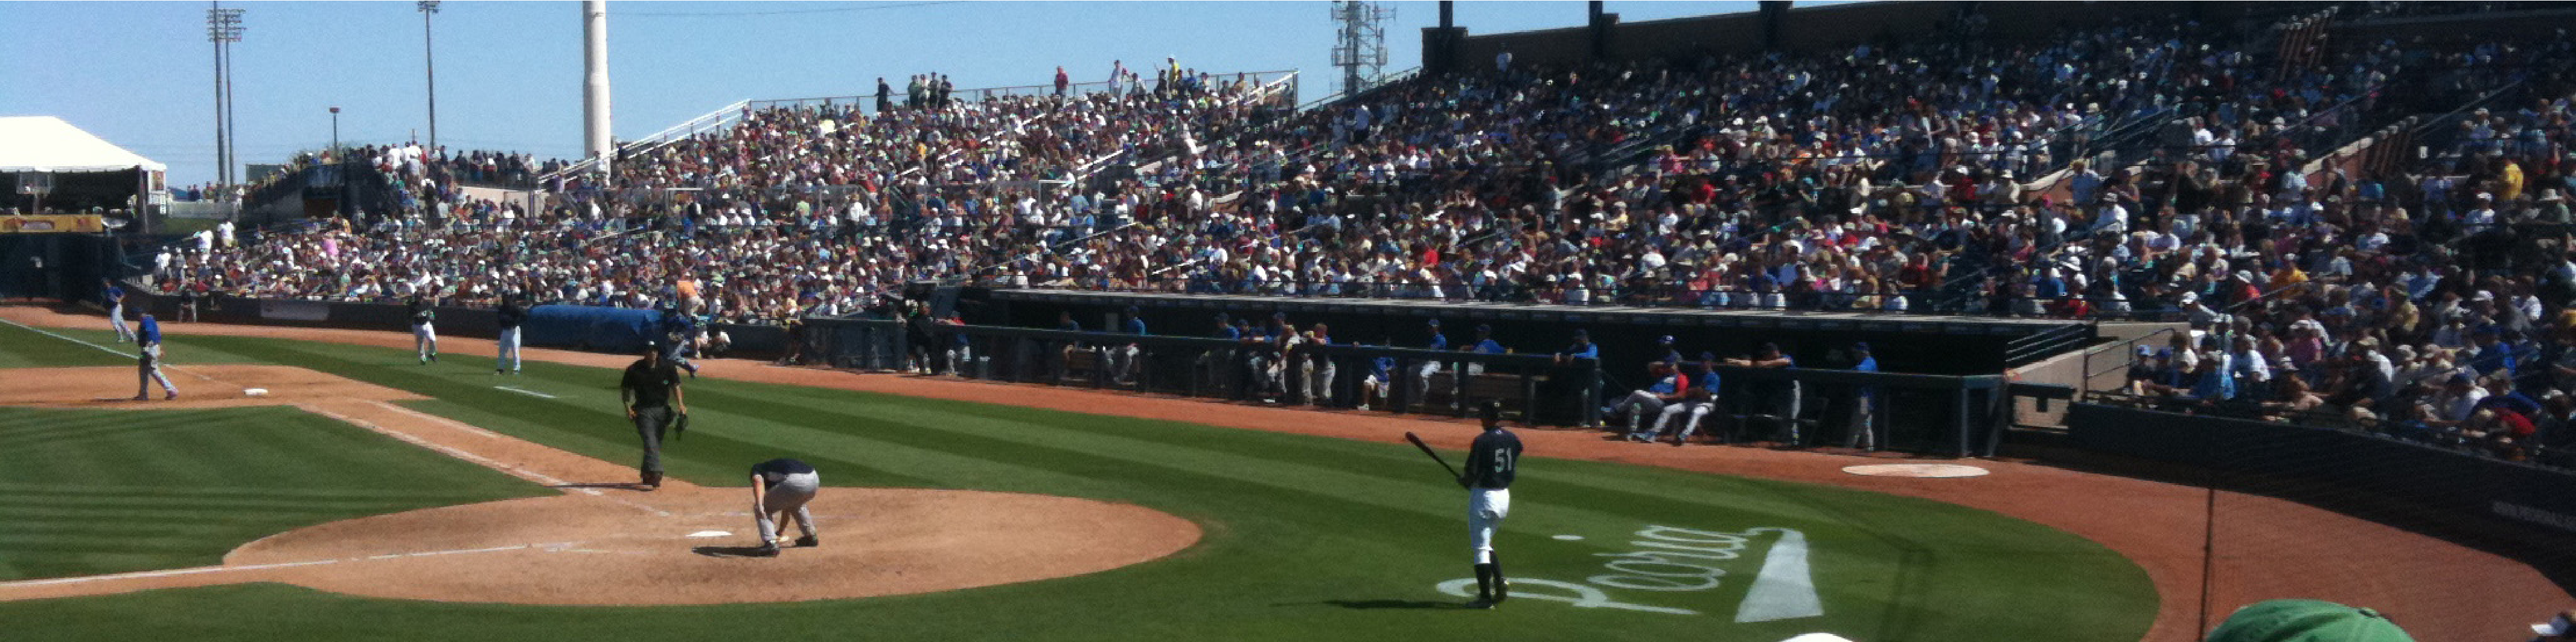
\includegraphics[width=\textwidth]{sampleteaser}
%   \caption{Seattle Mariners at Spring Training, 2010.}
%   \Description{Enjoying the baseball game from the third-base
%   seats. Ichiro Suzuki preparing to bat.}
%   \label{fig:teaser}
% \end{teaserfigure}

%%
%% This command processes the author and affiliation and title
%% information and builds the first part of the formatted document.
\maketitle

\section{Introduction}
 We revisit the famous methods simaltanously discovered by Dandelin, Lobachevsky, and Graeffe (See \cite{10.2307/2310626} for a history of this problem) and and make furhter progress by applying this indentity to the problem of approximating the root radius of a polynomial.
This is a key step in many sub-division based root finding algorithms.
One of the novelties of our algorithm is the Rational Root Tree Algorithm, \emph{i.e.,} Alg.~\ref{alg:circ_roots_rational_form}, which allows one to compute the angles of the iterated $2^\mathrm{th}$ roots in Eq.~\ref{eqdndrt0} with exact percision over the rationals; thus, greatly reducing the numerical stability Eq.~\ref{eqdndrt0} since, as we will see in Sec.~\ref{sec:the_ana} (as well as Thm.~\ref{thm:rat_root_correctness}), the most numerically unstable steps in Eq.~\ref{eqdndrt0} is the computation of the roots $x^{\frac{1}{2^m}}$.
Another advantage of our algorithm is that it assumes the blackbox polynomial model; \emph{i.e.,}, our algorithm works under the stronger assumption that one only compute $p(x)$ via some oracle.
We give both theoritical gaurentess in Sec.~\ref{sec:the_ana} and empirical evidence in Sec.~\ref{sec:exp} that our algorithm performs well.

\section{Related Works}
The main method for rootfinding by root-squaring was simaltanously discovered by Dandelin, Lobachevsky, and Graeffe in the 19$^\mathrm{th}$ century (See \cite{10.2307/2310626}). Two of the first works to consider algorithms based on the formulae for modern computers were \cite{10.1145/321186.321198} and \cite{10.1145/364955.364974}; the later of which gave explicit pseudocode for the a rootfinding algorithm that uses Eq.~\ref{eqdnd}.
The work \cite{Malajovich2001OnTG} also considers rootfinding using Eq.~\ref{eqdnd} and further state that the DLG method becomes very unstable for $\ell > 2$; by contrast, as we will see in Sec.~\ref{sec:exp}, our algorithm performs reasonably well for $\ell$ as large as $12$.
The same authors went on design a variation of the DLG rootfinding algorithm that makes use of different renomalizations and other preprocessing tranformations for DLG root finding in \cite{Malajovich2001TangentGI}, the work also proves convergence results for their DLG iterative algorithm.
The authors of \cite{Bialas2010GeneralizationOV} consider DLG based algorithms for the solutions of fractional-order polynomials, \emph{i.e.,} generalized polynomials that have rational exponents. In \cite{Hoeven2011EfficientRC} the authors use apply the DLG formulae to root counting.
The authors of \cite{Grenet2015DeterministicRF} apply the DLG formulae to solving polynomials over finite fields. The authors of \cite{Becker2018ANS} apply DLG iterations to the benchmark problem (\emph{i.e.,}, the isolsation of the roots of a polynomials, See Sec.\ref{srrapp}) to improve upon the record bound in \cite{pan2002univariate} which at the time was unborken for 14 years.
This short survey illustrates that the the application of the DLG to root finding (while more than a centuary old) is still an interesting research topic.
One of the novelties and improvements of our algorithms is to consider the identies given by Eq.~\ref{eqdndrt}, instead of the usual Eq.\ref{eqdnd}, to approximating the root radius.
Furthermore, we show that, contrary to intuition, our algorithm is numerical stable and well behaved when taking the limit of Eq.~\ref{eqdndrt} to 0.


\section{Background and Motivation}\label{srrapp}
% %------------------------------------------------------------------------------
% \subsection{Root radius and root-squaring}\label{srrapp}
%
% %------------------------------------------------------------------------------.
% The algorithm of Sec. \ref{scnttstB1} and
%  \ref{scnttstB} only ensures
%  approximation of a root radius
% within  factors  of  $d^{1.25}$ and
% $d^{4.75}/m$, respectively (see   Algs.  \ref{algscrincl}$m$ and \ref{algscrcmpr}), versus  a factor of $5^{1/N}$ for, say, $N=3$  ensured by Thm. \ref{thtrn}, and this  is translated into the same error factors for estimated rigidity of the output disc.
% The  difference little affects our estimates for the overall cost of subdivision root-finders (see part (c) of Remark
% \ref{recmprlg}), but not so in some other important applications, e.g., in the following two cases:
% \begin{itemize}
% \item
% A disc $D(c,\rho)$ contains  a root if and only if
% $r_d(c,p)\le \rho$.
% \item
%  The estimates for $r_d(c,p')$  are
%   involved  in  path-lifting Newton's iterations (see  Myong-Hi Kim
%   and Scott Sutherland  \cite{KS94}).
% \end{itemize}
%
% %We also uses a disc $D(c,\alpha r_1(c,p))$ for
% %%\alpha\ge 1$ to initialize  subdivision
% %and Newton's iterations for root-finding.
% This motivates the following problem:
% given
% a range $[\rho_-,\rho_+]$ for  the $m$th smallest root radius, $r_{d-m+1}$, narrow this range.
% We already addressed this problem
%  in Remark \ref{retrhob}, but next
 % We present the refinement of root radii  approximation, based on the classical technique of recursive root-squaring, which also enables us to relax restriction of Rule 2 of Sec. \ref{ssbdbrf} on softness of exclusion test and to increase isolation of a disc (see, e.g.,  Remark \ref{resmplini}).
\subsection{Dandelin, Lobachevsky, and Graeffe's Formaulae}\label{subsec:DLG_form}
 The common procedure for root radii  approximation, based on the classical technique of recursive root-squaring, is to first make an input polynomial $p(x)$ monic by scaling it and/or the variable
  $x$ and then
 apply $k$ DLG (that is, Dandelin's aka
Lobachevsky's or Gr{\"a}ffe's) root-squaring iterations
(cf. \cite{10.2307/2310626}),
\begin{equation}\label{eqdnd}
 p_0(x)=\frac{1}{p_d}p(x),~p_{i+1}(x)=(-1)^ dp_i(\sqrt x)
p_i(-\sqrt x),~i=0,1,\dots.\ell
\end{equation}
for a fixed positive integer $\ell$
(see Remark \ref{rescdnd} below).
The $i$th  iteration squares the roots of $p_i(x)$ and
consequently the root radii from the origin, as well as
the  isolation of the unit disc $D(0,1)$.
Then one approximates
the ratio  $\rho_+/\rho_-$, the new scaled ratio of the root radii, for the polynomial $p_{\ell}(x)$ within a factor of $\gamma$ and readily recovers the approximation of this ratio for $p_0(x)$ and
$p(x)$ within a factor of
$\gamma^{1/2^{\ell}}$.

Given the coefficients of
$p_i(x)$
we can reduce the $i$th root-squaring iteration, that is, the computation of
the coefficients of  $p_{i+1}(x)$, to polynomial multiplication and perform it in $O(d\log(d))$ arithmetic operations.
Unless the positive integer $\ell$ is small, the absolute values of the coefficients
of $p_{\ell}(x)$ vary  dramatically, and realistically one should either stop because of severe problems of numerical stability or apply the stable algorithm by Gregorio Malajovich and Jorge  P. Zubelli \cite{Malajovich2001OnTG}, which performs a single root-squaring at  arithmetic cost of order $d^2$.

For black box polynomials $p$, however, we apply
DLG iterations without computing
the coefficients, and the algorithm turns out to be quite efficient:
 for $\ell$ iterations  evaluate
 $p(x)$ at  $2^{\ell}$ equally spaced points  on a circle and obtain
 the values of the polynomial $p_{\ell}(x)=\prod\left(x-x_j^{2^{\ell}}\right)$
 at these $2^{\ell}$ points.

Furthermore,  evaluate the ratio
$p'(x)/p(x)=p_0'(x)/p_0(x)$
at these points by applying
the recurrence
 \begin{equation}\label{eqdndrt} \frac{p_{i+1}'(x)}{p_{i+1}(x)}=\frac{1}{2\sqrt x}\Big(\frac{p_{i}'(\sqrt x~)}{p_{i}(\sqrt x~)}-\frac{p_{i}'(-\sqrt x~)}{p_{i}(-\sqrt x~)}\Big),~i=0,1,\dots
\end{equation}
Recurrences (\ref{eqdnd}) and (\ref{eqdndrt}) reduce evaluation  of  $p_{\ell}(c)$ to the evaluation of $p(c)$ at  $q=2^{\ell}$  points
$c^{1/q}$ and  for $c\neq 0$ reduce evaluation  of
 the ratio
$p_{\ell}'(x)/p_{\ell}(x)$ at $x=c$ to the evaluation
of the ratio
$p'(x)/p(x)$ at the latter $q=2^{\ell}$ points $x=c^{1/q}$.
We will see that we can apply  recurrence (\ref{eqdndrt})
to support fast convergence to the convex hull of the roots.

% Clean

For $x=0$ recurrence (\ref{eqdndrt}) can be specialized as follows:
 \begin{equation}\label{eqdndrt0} \frac{p_{{\ell}}'(0)}{p_{\ell}(0)}=\Big(\frac{p_{\ell-1}'(x)}{p_{\ell-1}(x)}\Big)_{x=0}'=\Big(\frac{p'(x)}{p(x)}\Big)_{x=0}^{(\ell)},~\ell=1,2,\dots
\end{equation}
Notice an immediate extension:
\begin{equation}\label{eqdndrth} \frac{p_{{\ell}}^{(h)}(0)}{p_{\ell}(0)}=\prod_{g=1}^h\Big(\frac{p^{(g)}(x)}{p^{(g-1)}(x)}\Big)_{x=0}^{(\ell)},~h=1,2,\dots.
\end{equation}
Equations (\ref{eqdndrt0}) and more generally (\ref{eqdndrth})
enable us to  strengthen
upper estimates in Eq.~\ref{eq:rat_roo_radii_1} \& Eq.~\ref{eq:rat_roo_radii_2}
and more generally Eq.~\ref{eq:last_appen} for root-radii $r_j(0,p)$   at the origin  because $r_j(0,p_{\ell})=r_j(0,p)^{2^{\ell}}$ for $j=1,\dots,d$ (see  Eq.~\ref{eq:rat_roo_radii_1} \& Eq.~\ref{eq:rat_roo_radii_2}); we can  approximate the higher order derivatives
$\Big(\frac{p^{(g)}(x)}{p^{(g-1)}(x)}\Big)^{(\ell)}$
 at $x=0$ by following Remark.~\ref{rem:fin_diff}.
Besides the listed applications of
root-squaring, one can apply DLG to randomized exclusion tests for sparse polynomial.
One can apply root-squaring $p(x)\mapsto p_{\ell}(x)$ to improve  the error bound for the approximation of the power sums of the roots of  $p(x)$ in the unit disc $D(0,1)$ by Cauchy sums, but the improvement is about as much and at the same additional cost as by increasing the number $q$ of points of evaluation of the ratio $\frac{p'}{p}$.
\begin{remark}\label{rescdnd}
 One can approximate the leading coefficient $p_d$  of a black box polynomial $p(x)$. This coefficient is not involved in recurrence (\ref{eqdndrt}),
 and one can apply  recurrence (\ref{eqdnd}) by using a crude
 approximation to  $p_d$
 and if needed can scale polynomials
 $p_i(x)$ for some $i$.
\end{remark}

% Part 2 back
\subsection{Extremal root radii}\label{sec:ext_root_rad}

We cover some known estimates for extremal root radii in Sec.~\ref{subsec:class_est}. The most used estimates (Eq.~\ref{eq:last_appen} for $i=1$ and $c=0)$ readily follow from straightforward algbraic manipluations of $p_\text{rev}:=p_d+p_{d-1}x^1+...+p_0x^d$:
\begin{equation}\label{eq:rat_roo_radii_1}
r_{d}(c, p) \leq d\left|\frac{p(c)}{p^{\prime}(c)}\right|
\end{equation}
\text { and }
\begin{equation}\label{eq:rat_roo_radii_2}
 r_{1}(c, p) \geq\left|\frac{p_{\mathrm{rev}}^{\prime}(c)}{d p_{\mathrm{rev}}(c)}\right| .
\end{equation}
% clean
We strengthen these estimates in the case of $c=0$ by recalling DLG rootsquaring iterations Eq.~\ref{eqdndrt} of Sec.~\ref{subsec:DLG_form} and Equation \ref{eqdndrt0}. This immediately implies the following extension of Eq.~\ref{eq:rat_roo_radii_1} \& Eq.~\ref{eq:rat_roo_radii_2} for $c=0$ and all non-negative integers $\ell$ :
\begin{equation}\label{eq:rat_roo_radii_3}
r_{d}(0, p)^{2^{\ell}} \leq d \left|\left(\frac{p^{\prime}(x)}{p(x)}\right)_{x=0}^{(\ell)}\right|^{-1}
\end{equation}
\text { and }
\begin{equation}\label{eq:rat_roo_radii_4}
r_{1}(0, p)^{2^{\ell}} \geq d^{-1}\left|\left(\frac{ p^{\prime}_{\text {rev }}(x)}{p_{\text {rev }}(x)}\right)_{x=0}^{(\ell)}\right|
\end{equation}
\begin{remark}\label{rem:fin_diff}
 Given a complex $c$ and a positive integer $\ell$ one can approximate the values at $x=c$ of $\left(p(x) / p^{\prime}(x)\right)^{(\ell)}$ for a black box polynomial $p(x)$ by using divided differences, by extending expressions $p^{(i+1)}(c)=\lim _{x \rightarrow c} \frac{p^{(i)}(x)-p^{(i)}(c)}{x-c}$ for $i=0,1, \ldots, \ell-1$ and based on the mean value theorem \cite{Boor1995DividedD}.
\end{remark}

For $\ell=1$ one can instead apply the algorithm supporting the following elegant theorem and implicit in its constructive proof; the complexity of straightforward recursive extension to $\ell=2,3, \ldots$ increases exponentially in $\ell$.

\begin{theorem}
Given an algorithm that evaluates a black box polynomial $p(x)$ at a point $x$ over a field $\mathcal{K}$ of constants by using $A$ additions and subtractions, $S$ scalar multiplications (that is, multiplications by elements of the field $\mathcal{K}$ ), and $M$ other multiplications and divisions, one can extend this algorithm to the evaluation at $x$ of both $p(x)$ and $p^{\prime}(x)$ by using $2 A+M$ additions and subtractions, $2 S$ scalar multiplications, and $3 M$ other multiplications and divisions.
\end{theorem}

\begin{proof}
\cite{Linnainmaa1976}, \cite{baur1983complexity} proves the theorem for any function $f\left(x_{1}, \ldots, x_{s}\right)$ that has partial derivatives in all its $s$ variables $x_{1}, \ldots, x_{s}$.
\end{proof}

Next we prove that estimates \ref{eq:rat_roo_radii_3} and \ref{eq:rat_roo_radii_4} are extremely poor for worst case inputs.

\begin{theorem}
The ratios $\left|\frac{p(0)}{p^{\prime}(0)}\right|$ and $\left|\frac{p_{\mathrm{rev}}(0)}{p_{\mathrm{rev}}^{\prime}(0)}\right|$ are infinite for $p(x)=x^{d}-h^{d}$, while $r_{d}(c, p)=r_{1}(c, p)=r_{d}\left(c, p_{\text {rev }}\right)=r_{1}\left(c, p_{\text {rev }}\right)=|h|$.
Proof. Observe that the roots $x_{j}=h \exp \left(\frac{(j-1) \mathbf{i}}{2 \pi d}\right)$ of $p(x)=x^{d}-h^{d}$ for $j=$ $1,2, \ldots, d$ are the $d$ th roots of unity up to scaling by $h$.
\end{theorem}

Clearly, the problem persists at the points $x$ where $p^{\prime}(x)$ and $p_{\text {rev }}^{\prime}(x)$ vanish; rotation of the variable $\mathcal{R}_a :p(x) \mapsto t(x)=p(a x)$ for $|a|=1$ does not fix it but shifts $\mathcal{T}_c : p(x) \mapsto t(x)=p(x-c)$ for $c \neq 0$ can fix it, thus enhancing the power of estimates \ref{eq:rat_roo_radii_3} and \ref{eq:rat_roo_radii_4}.
Furthermore,
$$
\frac{1}{r_{d}(c, p)} \leq \frac{1}{d}\left|\frac{p^{\prime}(c)}{p(c)}\right|=\frac{1}{d}\left|\sum_{j=1}^{d} \frac{1}{c-x_{j}}\right|
$$
by virtue of \ref{eq:rat_roo_radii_1} \& \ref{eq:rat_roo_radii_2}, and so the approximation to the root radius $r_{d}(c, p)$ is poor if and only if severe cancellation occurs in the summation of the $d$ roots, and similarly for the approximation of $r_{1}(c, p)$. Such cancellations only occur for a narrow class of polynomials $p(x)$, with a low probability under random root models, although it occurs for the polynomials $p(x)=x^{d}-h^{d}$ of Thm. 5 and with high probability for random polynomials of \cite{erdos1950distribution}.
% clean till here
% TODO: keep cleaning

% Part 3 back
\subsection{Classical estimates for extremal root radii}\label{subsec:class_est}

Next we recall some non-costly estimates known for the extremal root radii $r_{1}=r_{1}(0, p)$ and $r_{d}=r_{d}(0, p)$ in terms of the coefficients of $p$ (cf. \cite{kerimov1977applied}, \cite{mignotte1999polynomials}, and \cite{yap2000fundamental}) and the two parameters
\begin{equation}\label{eq:radii_at_origin_1}
\tilde{r}_{-}:=\min _{i \geq 1}\left|\frac{p_{0}}{p_{i}}\right|^{\frac{1}{i}}, \tilde{r}_{+}:=\max _{i \geq 1}\left|\frac{p_{d-i}}{p_{d}}\right|^{\frac{1}{i}}
\end{equation}
These bounds on $r_{1}$ and $r_{d}$ hold in dual pairs since $r_{1}(0, p) r_{d}\left(0, p_{\text {rev }}\right)=1$.
% (see equation (8) for $j=1$ ).
Furthermore, we have that
\begin{equation}\label{eq:radii_at_origin_2}
\frac{1}{d} \tilde{r}_{+} \leq r_{1}<2 \tilde{r}_{+}, \frac{1}{2} \tilde{r}_{-} \leq r_{d} \leq d \tilde{r}_{-},
\end{equation}
\begin{equation}\label{eq:radii_at_origin_3}
\tilde{r}_{+} \sqrt{\frac{2}{d}} \leq r_{1} \leq \frac{1+\sqrt{5}}{2} \tilde{r}_{+}<1.62 \tilde{r}_{+} \text {if } p_{d-1}=0,
\end{equation}
\begin{equation}\label{eq:radii_at_origin_4}
0.618 \tilde{r}_{-}<\frac{2}{1+\sqrt{5}} \tilde{r}_{-} \leq r_{d} \leq \sqrt{\frac{d}{2}} \tilde{r}_{-} \text {if } p_{1}=0,
\end{equation}
\begin{equation}\label{eq:radii_at_origin_5}
r_{1} \leq 1+\sum_{i=0}^{d-1}\left|\frac{p_{i}}{p_{d}}\right|, \frac{1}{r_{d}} \leq 1+\sum_{i=1}^{d}\left|\frac{p_{i}}{p_{0}}\right| .
\end{equation}
$M(p):=\left|p_{d}\right| \max _{j=1}^{d}\left\{1,\left|x_{j}\right|\right\}$ is said to be the Mahler measure of $p$, and so $M\left(p_{\text {rev }}\right):=\left|p_{0}\right| \max _{j=1}^{d}\left\{1, \frac{1}{\left|x_{j}\right|}\right\} .$ It holds that
\begin{equation}\label{eq:radii_at_origin_6}
r_{1}^{2} \leq \frac{M(p)^{2}}{\left|p_{d}\right|} \leq \max _{i=0}^{d-1}\left|\frac{p_{i}}{p_{d}}\right|^{2}, \frac{1}{r_{d}^{2}} \leq \frac{M\left(p_{\mathrm{rev}}\right)^{2}}{\left|p_{0}\right|^{2}} \leq \max _{i=1}^{d}\left|\frac{p_{i}}{p_{0}}\right|^{2}
\end{equation}
Theorem 167 supports very fast approximation of all root radii of $p$ at the origin at a very low cost, which complements estimates \ref{eq:radii_at_origin_1}, \ref{eq:radii_at_origin_2} \ref{eq:radii_at_origin_3}, \ref{eq:radii_at_origin_4}, \ref{eq:radii_at_origin_5}, and \ref{eq:radii_at_origin_6}.

% Part 3.2 Background

One can extend all these bounds to the estimates for the root radii $r_{j}(c, p)$ for any fixed complex $c$ and all $j$ by observing that $r_{j}(c, p)=r_{j}(0, t)$ for the polynomial $t(x)=p(x-c)$ and applying Taylor's shift; \emph{i.e.,} applying the mapping $\mathcal{S}_{c ,\rho }:p(x) \mapsto p\left( \frac{x - c}{\rho} \right)$.

The algorithms in Sec.~\ref{sec:alg_des} closely approximate root radii $r_{j}(c, p)$ for a black box polynomial $p$ and a complex point $c$ at reasonably low cost, but the next well-known upper bounds on $r_{d}$ and lower bounds on $r_{1}$ (cf. \cite{kerimov1977applied},\cite{carstensen1991inclusion},\cite{pan2000approximating},\cite{bini2000design}, and \cite{bini2014solving}) are computed at even a lower cost, defined by a single fraction $\frac{p_{0}}{p_{i}}$ or $\frac{p_{d-i}}{p_{d}}$ for any $i$, albeit these bounds are excessively large for the worst case input.
Finally, we have that
$r_{d} \leq \rho_{i,-}:=\left(\left(\begin{array}{c}d \\ i\end{array}\right)\left|\frac{p_{0}}{p_{i}}\right|\right)^{\frac{1}{i}}, \frac{1}{r_{1}} \leq \frac{1}{\rho_{i,+}}:=\left(\left(\begin{array}{l}d \\ i\end{array}\right)\left|\frac{p_{d}}{p_{d-i}}\right|\right)^{\frac{1}{i}}$
and therefore, since $p^{(i)}(0)=i ! p_{i} \text { for all } i>0$, that
\begin{equation}\label{eq:last_appen}
r_{d} \leq \rho_{i,-}=\left(i !\left(\begin{array}{c}
d \\
i
\end{array}\right)\left|\frac{p(0)}{p^{(i)}(0)}\right|\right)^{\frac{1}{i}}, \frac{1}{r_{1}} \leq \frac{1}{\rho_{i,+}}=\left(i !\left(\begin{array}{c}
d \\
i
\end{array}\right)\left|\frac{p_{\text {rev }}(0)}{p_{\text {rev }}^{(i)}(0)}\right|\right)^{\frac{1}{i}}
\end{equation}
for all $i$; from which we obtain relations \ref{eq:rat_roo_radii_1} and \ref{eq:rat_roo_radii_2} for $i=1$.

\section{Motivating Example}

\begin{figure}[h]
  \centering
  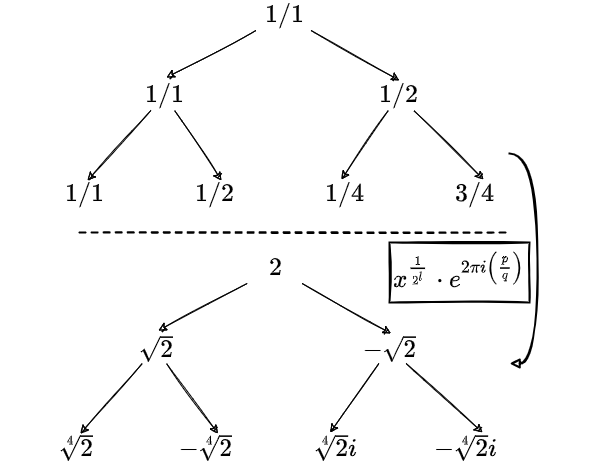
\includegraphics[width=\linewidth]{rational_root_tree.png}
  \caption{The upper tree depicts the steps of \textsc{\textsc{Circle\_Roots\_Rational\_Form}}($p,q,l$) in Alg.\ref{alg:circ_roots_rational_form} for $l=2$, $p=1$, and $q=1$. The lower tree depicts the steps of \textsc{Roots}($r,t,u,l$) in Alg.\ref{alg:roots} for $r=2$, $l=2$, $p=1$, and $q=1$}\label{fig:rat_roots_tree}
  \Description{}
\end{figure}

\begin{figure}[h]
  \centering
  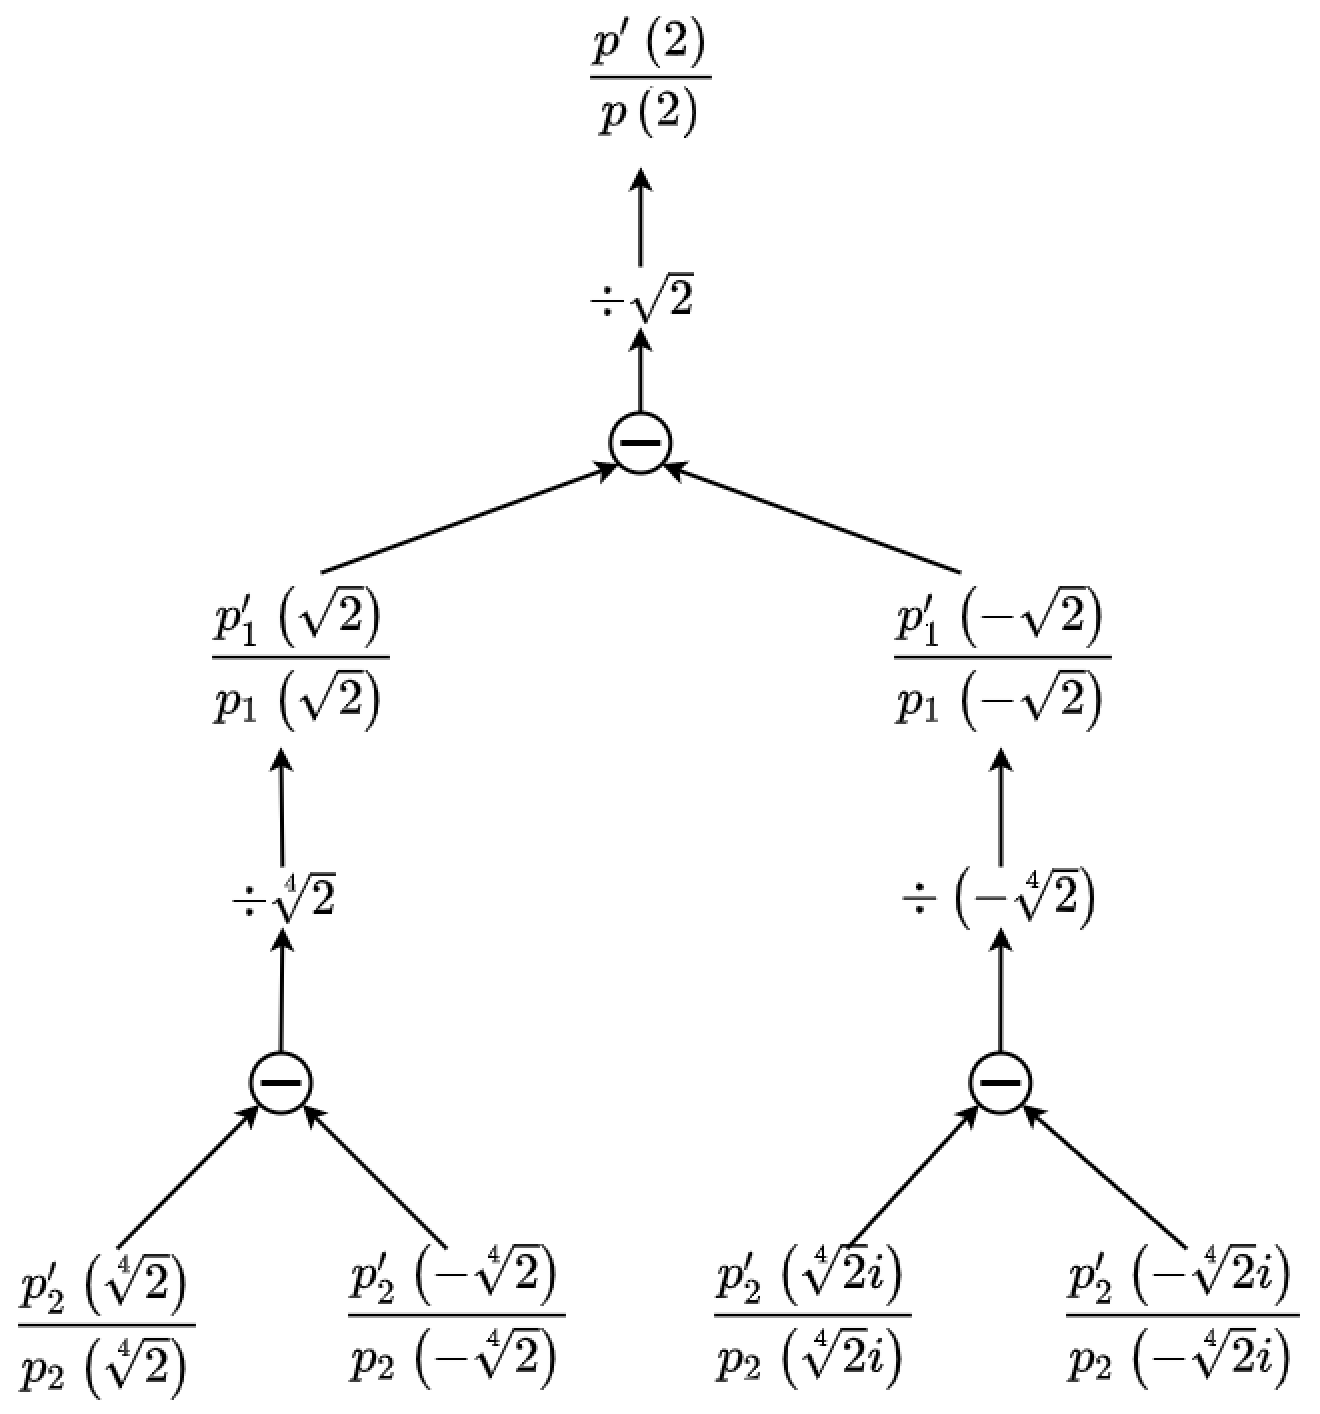
\includegraphics[width=\linewidth]{p_prime.png}
  \caption{The steps of \textsc{DLG\_Rational\_Rorm}($p,p^\prime,r,t,u,l$) in Alg.\ref{alg:DLG_rational_form} for $r=2$, $l=2$, $t=1$, and $u=1$.}\label{fig:DLG}
  \Description{}
\end{figure}



\section{Algorithm Design}\label{sec:alg_des}

In this section give the design of the general algorithm for approximating the root radius given by Eq.~\ref{eqdndrt0}.
There are two main steps: 1) going down the rational root tree, \emph{i.e.,} performing Alg.~\ref{alg:circ_roots_rational_form}, and 2) going up the rational root tree, \emph{i.e.,} performing Alg.~\ref{alg:DLG_rational_form}.
The going-down is depicted in Fig.~\ref{fig:rat_roots_tree} and the going-up is depicted in Fig.~\ref{fig:DLG}.
The other procedures are simple bookkeeping/preprocessing steps in between the two main going-down/going-up steps.
In particular we
1) first convert a complex number $x$ into polar coordinates $r,\theta$ where $\theta \approx \frac{p}{q} = \frac{p}{2^\epsilon}$, \emph{i.e.,} perform Alg.~\ref{alg:rational_angle_approx},
2) we then perform the first going down pass which gives the rational angles for the roots of $x$ in fraction form, \emph{i.e.,} perform Alg.~\ref{alg:circ_roots_rational_form},
3) we then perform the second pass of the going down algorithm where we compute the values $|x|^{\frac{1}{2^m}} \exp(2 \pi i \frac{p}{q})$ at the $m^\mathrm{th}$ level, and
4) finally, we then compute the values given by Eq.~\ref{eqdndrt} going back up the rational root tree.

\begin{algorithm}
   \caption{\textsc{Circle\_Roots\_Rational\_Form}($p,q,l$)}
   \label{alg:circ_roots_rational_form}
\begin{algorithmic}
\IF{ $p\%q$ == 0}
  \STATE  $r, s$ := (1,1)
\ELSE
  \STATE  $r, s$ := ($p$,$2q$)
\ENDIF
  \IF{ r\%s == 0}
    \STATE $t, u$ := (1,2)
  \ELSE
    \STATE $t, u$ := $(2r+s, 2s)$
  \ENDIF
	  \IF{$l$ == 1}
		  \RETURN [($r,s$),($t,u$)]
	\ELSIF {$l$ != 0}
		\STATE left  := \textsc{Circle\_Roots\_Rational\_Form}($r,s,l-1$)
		\STATE right := \textsc{Circle\_Roots\_Rational\_Form}($t,u,l-1$)
		\RETURN left $\cup$ right
	\ELSE
		\RETURN  [($p,q$)]
      \ENDIF
\end{algorithmic}
\end{algorithm}

The intuition behind Algorithm.~\ref{alg:circ_roots_rational_form} is that the square root operation satisfies
\begin{equation}\label{eq:rat_sq_imag}
p \% q \neq  0 \implies   \sqrt{\exp \left(2 \pi i \frac{p}{q}\right)}  = \exp \left(2 \pi i \frac{p}{2q}\right)
\end{equation}
and
\begin{equation}\label{eq:rat_sq_real}
p \% q = 0 \implies   \sqrt{\exp \left(2 \pi i \frac{1}{1}\right)}  = \exp \left(2 \pi i \frac{1}{1}\right) = 1,
\end{equation}
and the negation operation satisfies
\begin{equation}\label{eq:rat_neg_imag}
p \% q \neq  0 \implies   -\exp \left(2 \pi i \frac{r}{s}\right)  = \exp \left(2 \pi i \frac{2r+s} {2s}\right)
\end{equation}
and
\begin{equation}\label{eq:rat_neg_real}
p \% q = 0 \implies   \sqrt{\exp \left(2 \pi i \frac{1}{1}\right)}  = \exp \left(2 \pi i \frac{1}{2}\right) = -1;
\end{equation}
thus, the first four lines of Algorithm.~\ref{alg:circ_roots_rational_form} computes the (angle of the) positive square root, $\sqrt{x}$, of complex number on the unit circle and the next four lines Alg.~\ref{alg:circ_roots_rational_form} computes the (angle of the) negative square root, $-\sqrt{x}$. Therefore, we have:
\begin{theorem}\label{thm:rat_root_correctness}
  For a complex number, $x$, with a rational angle, \emph{i.e.,} $x = |x|\exp \left(2 \pi i \frac{p}{q}\right)$, Alg.~\ref{alg:circ_roots_rational_form} correctly computes the roots in Eq.~\ref{eqdndrt}.
\end{theorem}
\begin{proof}
Equation \ref{eq:rat_sq_imag}, \ref{eq:rat_sq_real}, \ref{eq:rat_neg_imag}, and \ref{eq:rat_neg_real} give the base case and the theorem follows by a straightforward induction.
\end{proof}


\begin{algorithm}
\caption{\textsc{Roots}($r,t,u,l$)}
\label{alg:roots}
\begin{algorithmic}
\STATE root\_tree = \textsc{Circle\_Roots\_Rational\_Form}($p,q,l$)
\STATE circ\_root = [$\exp\left(2\cdot\pi\cdot i \cdot \frac{r}{s}\right)$ for $r,s$ in root\_tree]
% \STATE circ\_root       = circ\_roots($t,u,l$)
\STATE roots =[$\sqrt[2^l]{r}\cdot$root for root in circ\_root]
\RETURN roots
\end{algorithmic}
\end{algorithm}


% \begin{algorithm}
%    \caption{circ\_roots\_rational\_form($p,q,l$)}
%    \label{alg:circ_roots_rational_form}
% \begin{algorithmic}
%   \STATE $r, s$  := angle\_sq\_root($p,q$)
% 	\STATE $t, u$  := angle\_neg($r,s$)
% 	  \IF{$l$ == 1}
% 		  \RETURN [($r,s$),($t,u$)]
% 	\ELSIF {$l$ != 0}
% 		\STATE left  := circ\_roots\_rational\_form($r,s,l-1$)
% 		\STATE right := circ\_roots\_rational\_form($t,u,l-1$)
% 		\RETURN left $\cup$ right
% 	\ELSE
% 		\RETURN  [($p,q$)]
%       \ENDIF
% \end{algorithmic}
% \end{algorithm}


% \begin{algorithm}
% \caption{angle\_sq\_root(p,q)}
% \label{alg:angle_sq_root}
% \begin{algorithmic}
% 	\IF{ $p\%q$ == 0}
% 		\RETURN  (1,1)
% 	\ELSE
% 		\RETURN  ($p$,$2q$)
%   \ENDIF
% \end{algorithmic}
% \end{algorithm}
%
%
% \begin{algorithm}
% \caption{angle\_neg(p,q)}
% \label{alg:angle_neg}
% \begin{algorithmic}
% 	\IF{ p\%q == 0}
% 		\RETURN  (1,2)
% 	\ELSE
% 		\RETURN  $(2p+q, 2q)$
%   \ENDIF
% \end{algorithmic}
% \end{algorithm}




% \begin{algorithm}
% \caption{circ\_roots($p,q,l$):}
% \label{alg:circ_roots}
% \begin{algorithmic}
% \STATE roots = circ\_roots\_rational\_form($p,q,l$)
% \RETURN [$\exp\left(2\cdot\pi\cdot i \cdot \frac{r}{s}\right)$ for r,s in roots]
% \end{algorithmic}
% \end{algorithm}





% \clearpage

\begin{algorithm}
\caption{\textsc{DLG\_Rational\_Form}($p,p^\prime,r,t,u,l$)}
\label{alg:DLG_rational_form}
\begin{algorithmic}
\STATE 	root      := \textsc{Roots}($r,t,u,l$)
\FOR {$r_i \in $ root}
\STATE 	base\_step[$i$] := $\frac{p^\prime(r_i)}{p(r_i)}$
\ENDFOR
\STATE  diff[0]   := base\_step
\FOR {$i \leq l$}
\FOR {$j \leq 2^{l-i-1}$}
\STATE 			diff[$i+1$][$j$]:=$\frac{1}{2}\frac{\text{diff}[i][2j]-\text{diff}[i][2j+1]}{\text{root}[2j]}$
\STATE 		root = roots($r,t,u,l-1-i$)
\ENDFOR
\ENDFOR
\RETURN diff$[l][0]$
\end{algorithmic}
\end{algorithm}





\begin{algorithm}
\caption{\textsc{DLG}($p,p^\prime,l,x, \epsilon$)}
\label{alg:rational_angle_approx}
\begin{algorithmic}
\STATE angle     := $\frac{1}{2\pi i} \log (x)$
\STATE $u $    := $2^{\epsilon}$
\STATE$t$      :=  $(\text{angle} \cdot u)\% 1$
\STATE $r$      := $|x|$
\RETURN \textsc{DLG\_Rational\_Form}($p,p^\prime,r,t,u,l$)
\end{algorithmic}
\end{algorithm}

%
% u     = pod(2,epsilon)
% t     = mp.fmod(angle,pod(2,-epsilon))
% r     = mpf(mp.fabs(x))




% def DLG_rational_form(p,dp,r,t,u,l):
% 	root       = roots(r,t,u,l)
% 	base_step  = [dp(r)*np.reciprocal(p(r)) for r in root]
% 	derivs     = [base_step]
% 	for i in range(l):
% 		derivs.append([])
% 		for j in range(2**(l-i-1)):
% 			derivs[i+1].append((np.reciprocal(root[2*j])/2)*(derivs[i][2*j] - derivs[i][2*j+1]))
% 		root = roots(r,t,u,l-1-i)
% 	return derivs[l][0]







% TODO: short discussion on stabilty
\section{Theoretical Analysis}\label{sec:the_ana}
% \newpage
% \clearpage
% \begin{lemma}
% The (relative) condition number operator satisifies the following properties:
% \begin{enumerate}
%   \item $\kappa\{f\} (x) = |x \log'(f(x)) |$
%   \item $\kappa\{f-g\}(x) = |x \frac{ \kappa \{f\}(x)- \kappa \{g\}(x) }{f(x)-g(x)}| $
%   \item $\kappa \left\{\frac{f}{g}\right\} (x)= ||\kappa\{ f\} (x)| - |\kappa\{ g\} (x)||$
%   \item $\kappa \left\{ f \circ g \right\}(x) = \left| |\kappa\{f\} (g(x) )\cdot \kappa\{g\} (x)|\right| $
% \end{enumerate}
% \end{lemma}
% \begin{theorem}
%   The condition number for $\frac{p_l'}{p_l}$ using
% \end{theorem}
\begin{theorem}
Algorithm.~\ref{alg:DLG_rational_form} performs $q \log q$ floating point subtractions, divisions, and multiplications and $q \log q$ applications of $\sin$ and $\cos$, where $q = 2^l$; furthermore, Algorithm.~\ref{alg:DLG_rational_form} performs at most $Cq \log q$  integer additions, ``multiplications-by-2'', and $ \%2^\epsilon $ (\emph{i.e.,} mod $ 2^\epsilon $) operations, where $C=1,3,2$ respectively.
\end{theorem}

\begin{theorem}
The $q \log q$  integer additions, ``multiplications-by-2'', and $ \%2^\epsilon $ (\emph{i.e.,} mod $ 2^\epsilon $) operations in Algorithm.~\ref{alg:DLG_rational_form} have negligble overhead; more precisely, integer addtions are always additions of 2 $\epsilon$-bit integers and ``multiplications-by-2'' and $ \%2^\epsilon $ (\emph{i.e.,} mod $ 2^\epsilon $) operations have constant time overhead.
\end{theorem}
\section{Experimental Results}\label{sec:exp}

All experiments were run using Python 3.7.7 on MacOS 11.6.1 with 2.8 GHz Dual-Core Intel Core i5 with 8 GB memory.  The names of the polynomials are referencing the names of the test univariate polynomials included as part of the MPSolve package. `-' in the tables indicate the test was terminated before completion.

\begin{table*}[t]
\caption{Experimental Data for Chebyshev}
\label{tab:chebyshev}
\vskip -0.15in
\begin{center}
\begin{small}
\begin{sc}
\begin{tabular}{lccccccc}
\toprule
&  &  & mpmath & relative  & relative &  & mpsolve \\
degree  & $\ell$& $e=-\log(|x|)$& Precision &error $r_d$       & error $r_1$ &runtime& root radius\\
\midrule
 20 & 4 & 616 & 332 & 0.155 & 0.0939 & 0.27 & $[0.0785, 0.997]$\\
 40 & 5 & 616 & 332 & 0.0981 & 0.0589 & 1.13 & $[0.0393, 0.999]$\\
 80 & 6 & 617 & 334 & 0.0593 & 0.0353 & 5.26 & $[0.0196, 1.0]$\\
 160 & 7 & 617 & 334 & 2.71 & 0.0205 & 20.88 & $[0.00982, 1.0]$\\
 320 & 8 & 617 & 334 & 37.6 & 0.465 & 88.4 & $[0.00491, 1.0]$\\
\bottomrule
\end{tabular}
\end{sc}
\end{small}
\end{center}
\vskip 0.05in
\end{table*}

\begin{table*}[t]
\caption{Experimental Data for chromatic polynomial (zero root removed) kind a}
\label{tab:chrma}
\vskip -0.15in
\begin{center}
\begin{small}
\begin{sc}
\begin{tabular}{lccccccc}
\toprule
&  &  & mpmath & relative  & relative &  & mpsolve \\
degree  & $l$& $e=-\log(|x|)$& Precision &error $r_d$       & error $r_1$ &runtime& root radius\\
\midrule
 21 & 4 & 616 & 332 & 0.215 & 0.139 & 0.22 & $[1.0, 3.17]$\\
 341 & 8 & 617 & 334 & 0.717 & 0.547 & 105.48 & $[0.884, 3.41]$\\
 85 & 6 & 617 & 334 & 0.0369 & 0.0452 & 5.63 & $[1.0, 3.25]$\\
\bottomrule
\end{tabular}
\end{sc}
\end{small}
\end{center}
\vskip 0.05in
\end{table*}


\begin{table*}[t]
\caption{Experimental Data for chromatic polynomial deflated: a}
\label{tab:chrma_d}
\vskip -0.15in
\begin{center}
\begin{small}
\begin{sc}
\begin{tabular}{lccccccc}
\toprule
&  &  & mpmath & relative  & relative &  & mpsolve \\
degree  & $l$& $e=-\log(|x|)$& Precision &error $r_d$       & error $r_1$ &runtime& root radius\\
\midrule
20 & 4 & 616 & 332 & 0.16 & 0.175 & 0.26 & $[1.3, 3.01]$\\
 340 & 8 & 617 & 334 & 0.658 & 0.699 & 93.82 & $[0.741, 3.11]$\\
 84 & 6 & 617 & 334 & 0.0548 & 0.00507 & 5.53 & $[1.1, 3.06]$\\
\bottomrule
\end{tabular}
\end{sc}
\end{small}
\end{center}
\vskip 0.05in
\end{table*}


\begin{table*}[t]
\caption{Experimental Data for chromatic polynomial (zero root removed) kind c}
\label{tab:chrmc}
\vskip -0.15in
\begin{center}
\begin{small}
\begin{sc}
\begin{tabular}{lccccccc}
\toprule
&  &  & mpmath & relative  & relative &  & mpsolve \\
degree  & $l$& $e=-\log(|x|)$& Precision &error $r_d$       & error $r_1$ &runtime& root radius\\
\midrule
 22 & 4 & 616 & 332 & 0.211 & 0.138 & 0.3 & $[1.0, 3.03]$\\
 342 & 8 & 617 & 334 & 0.718 & 0.279 & 94.64 & $[0.897, 4.13]$\\
\bottomrule
\end{tabular}
\end{sc}
\end{small}
\end{center}
\vskip 0.05in
\end{table*}


\begin{table*}[t]
\caption{Experimental Data for chromatic polynomial deflated, kind c}
\label{tab:chrmc_d}
\vskip -0.15in
\begin{center}
\begin{small}
\begin{sc}
\begin{tabular}{lccccccc}
\toprule
&  &  & mpmath & relative  & relative &  & mpsolve \\
degree  & $l$& $e=-\log(|x|)$& Precision &error $r_d$       & error $r_1$ &runtime& root radius\\
\midrule
11 & 3 & 616 & 332 & 0.251 & 0.242 & 0.05 & $[1.27, 2.8]$\\
 43 & 5 & 616 & 332 & 0.101 & 0.0996 & 1.23 & $[1.02, 2.97]$\\
 171 & 7 & 617 & 334 & 0.268 & 1.13 & 22.05 & $[0.715, 3.07]$\\
 683 & 9 & 619 & 338 & 0.164 & 0.257 & 374.69 & $[0.519, 3.1]$\\
\bottomrule
\end{tabular}
\end{sc}
\end{small}
\end{center}
\vskip 0.05in
\end{table*}


\begin{table*}[t]
\caption{Experimental Data for Curz}
\label{tab:curz}
\vskip -0.15in
\begin{center}
\begin{small}
\begin{sc}
\begin{tabular}{lccccccc}
\toprule
             &       &                       & mpmath   & relative       & relative       &               & mpsolve \\
degree  & $l$ & $e=-\log(|x|)$ & Precision & error $r_d$ & error $r_1$ & runtime & root radius\\
\midrule
 20 & 4 & 616 & 332 & 0.156 & 0.854 & 0.21 & $[0.452, 1.15]$\\
 40 & 5 & 616 & 332 & 0.199 & 0.776 & 1.13 & $[0.379, 1.26]$\\
 80 & 6 & 617 & 334 & 0.086 & 0.227 & 5.49 & $[0.318, 1.34]$\\
 160 & 7 & 617 & 334 & 0.0385 & 0.509 & 20.79 & $[0.271, 1.38]$\\
\bottomrule
\end{tabular}
\end{sc}
\end{small}
\end{center}
\vskip 0.05in
\end{table*}


\begin{table*}[t]
\caption{Experimental Data for Easy}
\label{tab:easy}
\vskip -0.15in
\begin{center}
\begin{small}
\begin{sc}
\begin{tabular}{lccccccc}
\toprule
&  &  & mpmath & relative  & relative &  & mpsolve \\
degree  & $l$& $e=-\log(|x|)$& Precision &error $r_d$       & error $r_1$ &runtime& root radius\\
\midrule
 100 & 6 & 617 & 334 & 0.12 & 0.0809 & 6.35 & $[0.949, 0.98]$\\
 200 & 7 & 617 & 334 & 0.068 & 0.047 & 25.57 & $[0.971, 0.99]$\\
 400 & 8 & 617 & 334 & 0.0381 & 0.0265 & 104.47 & $[0.983, 0.995]$\\
 1600 &10& 619 & 338 & 0.01 & 0.00 & 2228.22 & $[0.995, 0.999]$\\ %old nonmemo version data
  3200 &11& 619 & 338 & 0.00 & - & - & $[0.997, 0.999]$\\ %did not finish
\bottomrule
\end{tabular}
\end{sc}
\end{small}
\end{center}
\vskip 0.05in
\end{table*}


\begin{table*}[t]
\caption{Experimental Data for Exp}
\label{tab:exp}
\vskip -0.15in
\begin{center}
\begin{small}
\begin{sc}
\begin{tabular}{lccccccc}
\toprule
&  &  & mpmath & relative  & relative &  & mpsolve \\
degree  & $l$& $e=-\log(|x|)$& Precision &error $r_d$       & error $r_1$ &runtime& root radius\\
\midrule
 50 & 5 & 616 & 332 & 3.76 & 0.126 & 1.48 & $[14.9, 39.4]$\\
100 & 6 & 617 & 334 & 0.367 & 0.0598 & 7.37 & $[28.9, 83.9]$\\
 200 & 7 & 617 & 334 & 0.714 & 0.839 & 28.22 & $[56.8, 176.0]$\\
 400 & 8 & 617 & 334 & 0.965 & 0.985 & 107.96 & $[113.0, 365.0]$\\
\bottomrule
\end{tabular}
\end{sc}
\end{small}
\end{center}
\vskip 0.05in
\end{table*}

\begin{table*}[t]
\caption{Experimental Data for Geom1}
\label{tab:geom1}
\vskip -0.15in
\begin{center}
\begin{small}
\begin{sc}
\begin{tabular}{lccccccc}
\toprule
&  &  & mpmath & relative  & relative &  & mpsolve \\
degree  & $l$& $e=-\log(|x|)$& Precision &error $r_d$       & error $r_1$ &runtime& root radius\\
\midrule
 10 & 3 & 616 & 332 & 0.334 & 0.25 & 0.05 & $[1.0, 1.0\text{e+}18]$\\
 15 & 3 & 616 & 332 & 0.403 & 1.0 & 0.08 & $[1.0, 1.0\text{e+}28]$\\
 20 & 4 & 616 & 332 & 0.206 & 1.0 & 0.28 & $[1.0, 1.0\text{e+}38]$\\
 40 & 5 & 616 & 332 & 0.122 & 1.0 & 1.18 & $[1.0, 1.0\text{e+}78]$\\
\bottomrule
\end{tabular}
\end{sc}
\end{small}
\end{center}
\vskip 0.05in
\end{table*}

\begin{table*}[t]
\caption{Experimental Data for Geom2}
\label{tab:geom2}
\vskip -0.15in
\begin{center}
\begin{small}
\begin{sc}
\begin{tabular}{lccccccc}
\toprule
&  &  & mpmath & relative  & relative &  & mpsolve \\
degree  & $l$& $e=-\log(|x|)$& Precision &error $r_d$       & error $r_1$ &runtime& root radius\\
\midrule
 10 & 3 & 616 & 332 & 0.334 & 0.25 & 0.06 & $[1.0\text{e-}18, 1.0]$\\
 15 & 3 & 616 & 332 & 8.09e+4 & 0.287 & 0.06 & $[1.0\text{e-}28, 1.0]$\\
 20 & 4 & 616 & 332 & 2.63e+26 & 0.171 & 0.23 & $[1.0\text{e-}38, 1.0]$\\
 40 & 5 & 616 & 332 & 1.61e+72 & 0.109 & 1.14 & $[1.0\text{e-}78, 1.0]$\\
\bottomrule
\end{tabular}
\end{sc}
\end{small}
\end{center}
\vskip 0.05in
\end{table*}

\begin{table*}[t]
\caption{Experimental Data for Geom3}
\label{tab:geom3}
\vskip -0.15in
\begin{center}
\begin{small}
\begin{sc}
\begin{tabular}{lccccccc}
\toprule
&  &  & mpmath & relative  & relative &  & mpsolve \\
degree  & $l$& $e=-\log(|x|)$& Precision &error $r_d$       & error $r_1$ &runtime& root radius\\
\midrule
 10 & 3 & 616 & 332 & 0.334 & 0.25 & 0.05 & $[9.54\text{e-}7, 0.25]$\\
 20 & 4 & 616 & 332 & 2.41 & 0.171 & 0.24 & $[9.09\text{e-}13, 0.25]$\\
 40 & 5 & 616 & 332 & 1.95e+18 & 0.109 & 1.15 & $[8.27\text{e-}25, 0.25]$\\
 80 & 6 & 617 & 334 & 1.83e+45 & 0.0662 & 5.73 & $[6.84\text{e-}49, 0.25]$\\
\bottomrule
\end{tabular}
\end{sc}
\end{small}
\end{center}
\vskip 0.05in
\end{table*}


\begin{table*}[t]
\caption{Experimental Data for Geom4}
\label{tab:geom4}
\vskip -0.15in
\begin{center}
\begin{small}
\begin{sc}
\begin{tabular}{lccccccc}
\toprule
&  &  & mpmath & relative  & relative &  & mpsolve \\
degree  & $l$& $e=-\log(|x|)$& Precision &error $r_d$       & error $r_1$ &runtime& root radius\\
\midrule
 10 & 3 & 616 & 332 & 0.334 & 0.25 & 0.05 & $[4.0, 1.05\text{e+}6]$\\
 20 & 4 & 616 & 332 & 0.206 & 0.707 & 0.27 & $[4.0, 1.1\text{e+}12]$\\
 40 & 5 & 616 & 332 & 0.122 & 1.0 & 1.15 & $[4.0, 1.21\text{e+}24]$\\
 80 & 6 & 617 & 334 & 0.0709 & 1.0 & 5.28 & $[4.0, 1.46\text{e+}48]$\\
\bottomrule
\end{tabular}
\end{sc}
\end{small}
\end{center}
\vskip 0.05in
\end{table*}

\begin{table*}[t]
\caption{Experimental Data for Hermite}
\label{tab:hermite}
\vskip -0.15in
\begin{center}
\begin{small}
\begin{sc}
\begin{tabular}{lccccccc}
\toprule
&  &  & mpmath & relative  & relative &  & mpsolve \\
degree  & $l$& $e=-\log(|x|)$& Precision &error $r_d$       & error $r_1$ &runtime& root radius\\
\midrule
 20 & 4 & 616 & 332 & 0.155 & 0.129 & 0.28 & $[0.245, 5.39]$\\
 40 & 5 & 616 & 332 & 0.0981 & 0.0876 & 1.31 & $[0.175, 8.1]$\\
 80 & 6 & 617 & 334 & 0.0593 & 0.0555 & 5.97 & $[0.124, 11.9]$\\
 160 & 7 & 617 & 334 & 0.0348 & 0.0335 & 23.56 & $[0.0877, 17.2]$\\
 320 & 8 & 617 & 334 & 2.08 & 0.785 & 88.88 & $[0.062, 24.7]$\\
\bottomrule
\end{tabular}
\end{sc}
\end{small}
\end{center}
\vskip 0.05in
\end{table*}

\begin{table*}[t]
\caption{Experimental Data for Kam1}
\label{tab:kam1}
\vskip -0.15in
\begin{center}
\begin{small}
\begin{sc}
\begin{tabular}{lccccccc}
\toprule
&  &  & mpmath & relative  & relative &  & mpsolve \\
degree  & $l$& $e=-\log(|x|)$& Precision &error $r_d$       & error $r_1$ &runtime& root radius\\
\midrule
 7 & 2 & 615 & 331 & 0.368 & 1.0 & 0.01 & $[3.0\text{e-}12, 15.8]$\\
 7 & 2 & 615 & 331 & 0.368 & 1.0 & 0.01 & $[3.0\text{e-}40, 1.0\text{e+}4]$\\
 7 & 2 & 615 & 331 & 2.37e+93 & 1.0 & 0.01 & $[3.0\text{e-}140, 1.0\text{e+}14]$\\
\bottomrule
\end{tabular}
\end{sc}
\end{small}
\end{center}
\vskip 0.05in
\end{table*}

\begin{table*}[t]
\caption{Experimental Data for Kam2}
\label{tab:kam2}
\vskip -0.15in
\begin{center}
\begin{small}
\begin{sc}
\begin{tabular}{lccccccc}
\toprule
&  &  & mpmath & relative  & relative &  & mpsolve \\
degree  & $l$& $e=-\log(|x|)$& Precision &error $r_d$       & error $r_1$ &runtime& root radius\\
\midrule
 9 & 3 & 616 & 332 & 0.107 & 1.0 & 0.03 & $[1.73\text{e-}6, 251.0]$\\
 9 & 3 & 616 & 332 & 0.107 & 1.0 & 0.03 & $[1.73\text{e-}20, 1.0\text{e+}8]$\\
 9 & 3 & 616 & 332 & 4.23e+46 & 1.0 & 0.03 & $[1.73\text{e-}70, 1.0\text{e+}28]$\\
\bottomrule
\end{tabular}
\end{sc}
\end{small}
\end{center}
\vskip 0.05in
\end{table*}

\begin{table*}[t]
\caption{Experimental Data for Kam3}
\label{tab:kam3}
\vskip -0.15in
\begin{center}
\begin{small}
\begin{sc}
\begin{tabular}{lccccccc}
\toprule
&  &  & mpmath & relative  & relative &  & mpsolve \\
degree  & $l$& $e=-\log(|x|)$& Precision &error $r_d$       & error $r_1$ &runtime& root radius\\
\midrule
 9 & 3 & 616 & 332 & 0.107 & 1.0 & 0.03 & $[1.73\text{e-}6, 251.0]$\\
 9 & 3 & 616 & 332 & 0.107 & 1.0 & 0.03 & $[1.73\text{e-}20, 1.0\text{e+}8]$\\
 9 & 3 & 616 & 332 & 4.23e+46 & 1.0 & 0.03 & $[1.73\text{e-}70, 1.0\text{e+}28]$\\
\bottomrule
\end{tabular}
\end{sc}
\end{small}
\end{center}
\vskip 0.05in
\end{table*}

\begin{table*}[t]
\caption{Experimental Data for Kir1}
\label{tab:kir1}
\vskip -0.15in
\begin{center}
\begin{small}
\begin{sc}
\begin{tabular}{lccccccc}
\toprule
&  &  & mpmath & relative  & relative &  & mpsolve \\
degree  & $l$& $e=-\log(|x|)$& Precision &error $r_d$       & error $r_1$ &runtime& root radius\\
\midrule
 44 & 5 & 616 & 332 & 4.41e-5 & 0.000443 & 1.28 & $[0.5, 0.5]$\\
  84 & 6 & 617 & 334 & 2.29e-5 & 0.000464 & 2.9 & $[0.5, 0.5]$\\
 164 & 7 & 617 & 334 & 1.16e-5 & 0.000476 & 9.79 & $[0.5, 0.5]$\\
 8 & 3 & 616 & 332 & 0.000244 & 0.000244 & 0.02 & $[0.5, 0.5]$\\ %symb
\bottomrule
\end{tabular}
\end{sc}
\end{small}
\end{center}
\vskip 0.05in
\end{table*}

\begin{table*}[t]
\caption{Experimental Data for Kir1 mod}
\label{tab:kir1_mod}
\vskip -0.15in
\begin{center}
\begin{small}
\begin{sc}
\begin{tabular}{lccccccc}
\toprule
&  &  & mpmath & relative  & relative &  & mpsolve \\
degree  & $l$& $e=-\log(|x|)$& Precision &error $r_d$       & error $r_1$ &runtime& root radius\\
\midrule
 44 & 5 & 616 & 332 & 0.000983 & 0.00095 & 1.26 & $[0.5, 0.5]$\\
 84 & 6 & 617 & 334 & 0.00364 & 0.00364 & 2.99 & $[0.498, 0.502]$\\
 164 & 7 & 617 & 334 & 0.00734 & 0.00749 & 10.35 & $[0.496, 0.504]$\\ %_mod
\bottomrule
\end{tabular}
\end{sc}
\end{small}
\end{center}
\vskip 0.05in
\end{table*}


\begin{table*}[t]
\caption{Experimental Data for  Lagurerre }
\label{tab:lagurerre}
\vskip -0.15in
\begin{center}
\begin{small}
\begin{sc}
\begin{tabular}{lccccccc}
\toprule
&  &  & mpmath & relative  & relative &  & mpsolve \\
degree  & $l$& $e=-\log(|x|)$& Precision &error $r_d$       & error $r_1$ &runtime& root radius\\
\midrule
 20 & 4 & 616 & 332 & 0.206 & 0.167 & 0.22 & $[0.0705, 66.5]$\\
 40 & 5 & 616 & 332 & 0.122 & 0.108 & 1.28 & $[0.0357, 142.0]$\\
 80 & 6 & 617 & 334 & 0.0709 & 0.0659 & 5.63 & $[0.018, 297.0]$\\
 160 & 7 & 617 & 334 & 3.09 & 0.954 & 22.21 & $[0.00901, 610.0]$\\
 320 & 8 & 617 & 334 & 41.4 & 0.996 & 89.64 & $[0.00451, 1.24\text{e+}3]$\\
\bottomrule
\end{tabular}
\end{sc}
\end{small}
\end{center}
\vskip 0.05in
\end{table*}

\begin{table*}[t]
\caption{Experimental Data for Lar1}
\label{tab:lar1}
\vskip -0.15in
\begin{center}
\begin{small}
\begin{sc}
\begin{tabular}{lccccccc}
\toprule
&  &  & mpmath & relative  & relative &  & mpsolve \\
degree  & $l$& $e=-\log(|x|)$& Precision &error $r_d$       & error $r_1$ &runtime& root radius\\
\midrule
 20 & 4 & 616 & 332 & 7.06e+9 & 1.0 & 0.1 & $[3.73\text{e-}22, 1.0\text{e+}50]$\\
 200 & 7 & 617 & 334 & 9.69e+19 & 0.311 & 0.83 & $[3.73\text{e-}22, 41.0]$\\
\bottomrule
\end{tabular}
\end{sc}
\end{small}
\end{center}
\vskip 0.05in
\end{table*}

\begin{table*}[t]
\caption{Experimental Data for Legendre}
\label{tab:legendre}
\vskip -0.15in
\begin{center}
\begin{small}
\begin{sc}
\begin{tabular}{lccccccc}
\toprule
&  &  & mpmath & relative  & relative &  & mpsolve \\
degree  & $l$& $e=-\log(|x|)$& Precision &error $r_d$       & error $r_1$ &runtime& root radius\\
\midrule
 20 & 4 & 616 & 332 & 0.155 & 0.0969 & 0.25 & $[0.0765, 0.993]$\\
 40 & 5 & 616 & 332 & 0.0981 & 0.0604 & 1.15 & $[0.0388, 0.998]$\\
 80 & 6 & 617 & 334 & 0.0593 & 0.0359 & 6.08 & $[0.0195, 1.0]$\\
  160 & 7 & 617 & 334 & 2.72 & 0.0637 & 19.97 & $[0.00979, 1.0]$\\
 320 & 8 & 617 & 334 & 37.7 & 0.456 & 81.12 & $[0.0049, 1.0]$\\
\bottomrule
\end{tabular}
\end{sc}
\end{small}
\end{center}
\vskip 0.05in
\end{table*}

\begin{table*}[t]
\caption{Experimental Data for LSR} %polynomial having roots with very large and very small moduli
\label{tab:lsr}
\vskip -0.15in
\begin{center}
\begin{small}
\begin{sc}
\begin{tabular}{lccccccc}
\toprule
&  &  & mpmath & relative  & relative &  & mpsolve \\
degree  & $l$& $e=-\log(|x|)$& Precision &error $r_d$       & error $r_1$ &runtime& root radius\\
\midrule
 24 & 4 & 616 & 332 & 2.88e+8 & 1.0 & 0.29 & $[1.0\text{e-}20, 1.0\text{e+}20]$\\
 52 & 5 & 616 & 332 & 1.81e+14 & 1.0 & 0.25 & $[1.0\text{e-}20, 1.0\text{e+}10]$\\ %lsr4_1
 52 & 5 & 616 & 332 & 1.81e+34 & 1.0 & 0.22 & $[1.0\text{e-}40, 1.0\text{e+}20]$\\ %lsr4_2
 52 & 5 & 616 & 332 & 1.81e+74 & 1.0 & 0.2 & $[1.0\text{e-}80, 1.0\text{e+}40]$\\ %lsr4_3
 224 & 7 & 617 & 334 & 3.62e+18 & 1.0 & 9.8 & $[1.0\text{e-}20, 1.0\text{e+}20]$\\
 500 & 8 & 617 & 334 & 1.92e+3 & 1.0 & 6.79 & $[0.0001, 2.0\text{e+}4]$\\
 500 & 8 & 617 & 334 & 5.77e+3 & 0.995 & 3.27 & $[3.33\text{e-}5, 1.0\text{e+}3]$\\
 500 & 8 & 617 & 334 & 1.05 & 1.0 & 3.05 & $[0.0916, 1.0\text{e+}200]$\\
\bottomrule
\end{tabular}
\end{sc}
\end{small}
\end{center}
\vskip 0.05in
\end{table*}


\begin{table*}[t]
\caption{Experimental Data for Mandelbrot}
\label{tab:mand}
\vskip -0.15in
\begin{center}
\begin{small}
\begin{sc}
\begin{tabular}{lccccccc}
\toprule
&  &  & mpmath & relative  & relative &  & mpsolve \\
degree  & $l$& $e=-\log(|x|)$& Precision &error $r_d$       & error $r_1$ &runtime& root radius\\
\midrule

\bottomrule
\end{tabular}
\end{sc}
\end{small}
\end{center}
\vskip 0.05in
\end{table*}

\begin{table*}[t]
\caption{Experimental Data for Mig1}
\label{tab:mig1}
\vskip -0.15in
\begin{center}
\begin{small}
\begin{sc}
\begin{tabular}{lccccccc}
\toprule
&  &  & mpmath & relative  & relative &  & mpsolve \\
degree  & $l$& $e=-\log(|x|)$& Precision &error $r_d$       & error $r_1$ &runtime& root radius\\
\midrule
 20 & 4 & 616 & 332 & 0.126 & 1.0 & 0.08 & $[0.01, 2.26]$\\
  50 & 5 & 616 & 332 & 0.0157 & 0.987 & 1.8 & $[0.00999, 1.83\text{e+}3]$\\
 100 & 6 & 617 & 334 & 0.0563 & 1.0 & 0.5 & $[0.01, 1.15]$\\
 100 & 6 & 617 & 334 & 0.0183 & 1.0 & 4.05 & $[0.01, 7.92]$\\
 200 & 7 & 617 & 334 & 2.66 & 1.0 & 0.8 & $[0.01, 1.07]$\\
 200 & 7 & 617 & 334 & 2.59 & 0.999 & 9.37 & $[0.01, 2.33]$\\
 500 & 8 & 617 & 334 & 18.2 & 0.99 & 1.59 & $[0.01, 1.03]$\\
\bottomrule
\end{tabular}
\end{sc}
\end{small}
\end{center}
\vskip 0.05in
\end{table*}


\begin{table*}[t]
\caption{Experimental Data for Mult}
\label{tab:mult}
\vskip -0.15in
\begin{center}
\begin{small}
\begin{sc}
\begin{tabular}{lccccccc}
\toprule
&  &  & mpmath & relative  & relative &  & mpsolve \\
degree  & $l$& $e=-\log(|x|)$& Precision &error $r_d$       & error $r_1$ &runtime& root radius\\
\midrule
 15 & 3 & 616 & 332 & 0.29 & 0.189 & 0.12 & $[0.869, 1.07]$\\
 20 & 4 & 616 & 332 & 0.0782 & 0.475 & 0.24 & $[0.01, 2.68]$\\
 22 & 4 & 616 & 332 & 0.213 & 0.105 & 0.24 & $[1.0, 20.0]$\\
  68 & 6 & 617 & 334 & 0.0566 & 0.0556 & 4.59 & $[0.25, 2.24]$\\
\bottomrule
\end{tabular}
\end{sc}
\end{small}
\end{center}
\vskip 0.05in
\end{table*}


\begin{table*}[t]
\caption{Experimental Data for $x^n - 1$}
\label{tab:nroots}
\vskip -0.15in
\begin{center}
\begin{small}
\begin{sc}
\begin{tabular}{lccccccc}
\toprule
&  &  & mpmath & relative  & relative &  & mpsolve \\
degree  & $l$& $e=-\log(|x|)$& Precision &error $r_d$       & error $r_1$ &runtime& root radius\\
\midrule

 50 & 5 & 616 & 332 & 5.18e+13 & 1.0 & 0.12 & $[1.0, 1.0]$\\
 100 & 6 & 617 & 334 & 7.06e+6 & 1.0 & 0.19 & $[1.0, 1.0]$\\
 200 & 7 & 617 & 334 & 2.69e+3 & 1.0 & 0.39 & $[1.0, 1.0]$\\
 400 & 8 & 617 & 334 & 50.5 & 0.981 & 0.79 & $[1.0, 1.0]$\\
 800 & 9 & 619 & 338 & 6.34 & 0.864 & 1.73 & $[1.0, 1.0]$\\
 1600 & 10 & 619 & 338 & 1.71 & 0.631 & 3.19 & $[1.0, 1.0]$\\
 3200 & 11 & 619 & 338 & 0.645 & 0.392 & 6.79 & $[1.0, 1.0]$\\
 6400 & 12 & 623 & 346 & 0.289 & 0.224 & 14.55 & $[1.0, 1.0]$\\
\bottomrule
\end{tabular}
\end{sc}
\end{small}
\end{center}
\vskip 0.05in
\end{table*}



\begin{table*}[t]
\caption{Experimental Data for $x^n - i$}
\label{tab:nrooti}
\vskip -0.15in
\begin{center}
\begin{small}
\begin{sc}
\begin{tabular}{lccccccc}
\toprule
&  &  & mpmath & relative  & relative &  & mpsolve \\
degree  & $l$& $e=-\log(|x|)$& Precision &error $r_d$       & error $r_1$ &runtime& root radius\\
\midrule
 50 & 5 & 616 & 332 & 4.94e+13 & 1.0 & 0.1 & $[1.0, 1.0]$\\
 100 & 6 & 617 & 334 & 7.07e+6 & 1.0 & 0.32 & $[1.0, 1.0]$\\
  200 & 7 & 617 & 334 & 2.69e+3 & 1.0 & 0.46 & $[1.0, 1.0]$\\
 400 & 8 & 617 & 334 & 50.5 & 0.981 & 0.85 & $[1.0, 1.0]$\\
 800 & 9 & 619 & 338 & 6.34 & 0.864 & 1.85 & $[1.0, 1.0]$\\
 1600 & 10 & 619 & 338 & 1.71 & 0.631 & 3.23 & $[1.0, 1.0]$\\
 3200 & 11 & 619 & 338 & 0.645 & 0.392 & 7.02 & $[1.0, 1.0]$\\
 6400 & 12 & 623 & 346 & 0.289 & 0.224 & 13.31 & $[1.0, 1.0]$\\
\bottomrule
\end{tabular}
\end{sc}
\end{small}
\end{center}
\vskip 0.05in
\end{table*}

\begin{table*}[t]
\caption{Experimental Data for Sendra}
\label{tab:sendra}
\vskip -0.15in
\begin{center}
\begin{small}
\begin{sc}
\begin{tabular}{lccccccc}
\toprule
&  &  & mpmath & relative  & relative &  & mpsolve \\
degree  & $l$& $e=-\log(|x|)$& Precision &error $r_d$       & error $r_1$ &runtime& root radius\\
\midrule
 160 & 7 & 617 & 334 & 0.658 & 2.14 & 24.34 & $[0.987, 2.01]$\\
 20 & 4 & 616 & 332 & 0.283 & 0.158 & 0.25 & $[0.9, 2.05]$\\
 320 & 8 & 617 & 334 & 0.809 & 1.64 & 88.08 & $[0.994, 2.0]$\\
 40 & 5 & 616 & 332 & 0.159 & 0.101 & 1.25 & $[0.95, 2.02]$\\
 80 & 6 & 617 & 334 & 0.287 & 0.573 & 5.2 & $[0.975, 2.01]$\\
\bottomrule
\end{tabular}
\end{sc}
\end{small}
\end{center}
\vskip 0.05in
\end{table*}

%\begin{table*}[t]
%\caption{Experimental Data for Sparse}
%\label{tab:sparse}
%\vskip -0.15in
%\begin{center}
%\begin{small}
%\begin{sc}
%\begin{tabular}{lccccccc}
%\toprule
%&  &  & mpmath & relative  & relative &  & mpsolve \\
%degree  & $l$& $e=-\log(|x|)$& Precision &error $r_d$       & error $r_1$ &runtime& root radius\\
%\midrule
%
%\bottomrule
%\end{tabular}
%\end{sc}
%\end{small}
%\end{center}
%\vskip 0.05in
%\end{table*}

\begin{table*}[t]
\caption{Experimental Data for Spiral}
\label{tab:spiral}
\vskip -0.15in
\begin{center}
\begin{small}
\begin{sc}
\begin{tabular}{lccccccc}
\toprule
&  &  & mpmath & relative  & relative &  & mpsolve \\
degree  & $l$& $e=-\log(|x|)$& Precision &error $r_d$       & error $r_1$ &runtime& root radius\\
\midrule
 10 & 3 & 616 & 332 & 5.1e-7 & 1.21e-6 & 0.05 & $[1.0, 1.0]$\\
 15 & 3 & 616 & 332 & 3.49e-7 & 1.15e-6 & 0.07 & $[1.0, 1.0]$\\
 20 & 4 & 616 & 332 & 4.55e-7 & 1.3e-6 & 0.23 & $[1.0, 1.0]$\\
 25 & 4 & 616 & 332 & 3.67e-7 & 1.25e-6 & 0.29 & $[1.0, 1.0]$\\
 30 & 4 & 616 & 332 & 3.08e-7 & 1.21e-6 & 0.41 & $[1.0, 1.0]$\\
\bottomrule
\end{tabular}
\end{sc}
\end{small}
\end{center}
\vskip 0.05in
\end{table*}




\begin{table*}[t]
\caption{Experimental Data for Toeplitz}
\label{tab:toep}
\vskip -0.15in
\begin{center}
\begin{small}
\begin{sc}
\begin{tabular}{lccccccc}
\toprule
&  &  & mpmath & relative  & relative &  & mpsolve \\
degree  & $l$& $e=-\log(|x|)$& Precision &error $r_d$       & error $r_1$ &runtime& root radius\\
\midrule
 128 & 7 & 617 & 334 & 0.0386 & 0.562 & 18.71 & $[1.31, 64.4]$\\
 256 & 8 & 617 & 334 & 0.0219 & 0.918 & 73.35 & $[1.34, 64.4]$\\
 128 & 7 & 617 & 334 & 0.0386 & 0.0272 & 17.68 & $[0.4, 13.2]$\\
 256 & 8 & 617 & 334 & 0.0225 & 0.599 & 72.66 & $[0.383, 13.2]$\\
\bottomrule
\end{tabular}
\end{sc}
\end{small}
\end{center}
\vskip 0.05in
\end{table*}


\begin{table*}[t]
\caption{Experimental Data for Wilk}
\label{tab:wilk}
\vskip -0.15in
\begin{center}
\begin{small}
\begin{sc}
\begin{tabular}{lccccccc}
\toprule
&  &  & mpmath & relative  & relative &  & mpsolve \\
degree  & $l$& $e=-\log(|x|)$& Precision &error $r_d$       & error $r_1$ &runtime& root radius\\
\midrule
 20 & 4 & 616 & 332 & 0.206 & 0.141 & 0.22 & $[1.0, 20.0]$\\
 30 & 4 & 616 & 332 & 0.237 & 0.0859 & 0.33 & $[1.0, 319.0]$\\
 40 & 5 & 616 & 332 & 0.122 & 0.0927 & 1.27 & $[1.0, 40.0]$\\
 80 & 6 & 617 & 334 & 0.0709 & 0.121 & 5.59 & $[1.0, 80.0]$\\
 160 & 7 & 617 & 334 & 0.0404 & 0.824 & 21.82 & $[1.0, 160.0]$\\
 320 & 8 & 617 & 334 & 0.0228 & 0.983 & 89.77 & $[1.0, 320.0]$\\
\bottomrule
\end{tabular}
\end{sc}
\end{small}
\end{center}
\vskip 0.05in
\end{table*}

\section{Conclusion}

%%
%% The acknowledgments section is defined using the "acks" environment
%% (and NOT an unnumbered section). This ensures the proper
%% identification of the section in the article metadata, and the
%% consistent spelling of the heading.
% \begin{acks}
% To Robert, for the bagels and explaining CMYK and color spaces.
% \end{acks}

%%
%% The next two lines define the bibliography style to be used, and
%% the bibliography file.
\bibliographystyle{ACM-Reference-Format}
\bibliography{ref.bib}

%%
%% If your work has an appendix, this is the place to put it.
\appendix



\end{document}
\endinput



%% template
\begin{table*}[t]
\caption{Experimental Data for }
\label{tab:template}
\vskip -0.15in
\begin{center}
\begin{small}
\begin{sc}
\begin{tabular}{lccccccc}
\toprule
&  &  & mpmath & relative  & relative &  & mpsolve \\
degree  & $l$& $e=-\log(|x|)$& Precision &error $r_d$       & error $r_1$ &runtime& root radius\\
\midrule
   20 &  &  &  &  &  &  & $[,]$ \\
   40 &  &  &  &  &  &  & $[,]$\\
   80 &  &  &  &  &  &  & $[,]$\\
 160 &  &  &  &  &  &  & $[,]$\\
 320 &  &  &  &  &  &  & $[,]$\\
\bottomrule
\end{tabular}
\end{sc}
\end{small}
\end{center}
\vskip 0.05in
\end{table*}
% \begin{figure}[h]
%   \centering
%   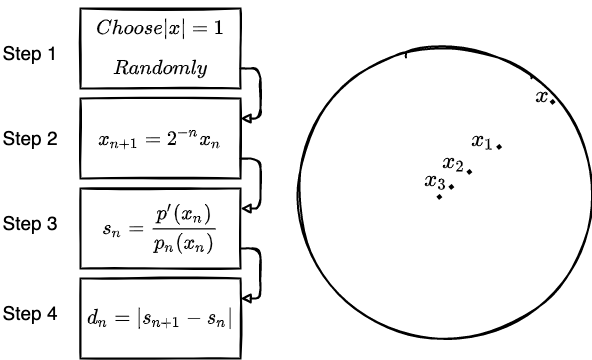
\includegraphics[width=\linewidth]{limit_test.png}
%   \caption{Limit test.}
%   \Description{The procedure for taking the limit to zero.}
% \end{figure}




%%
%% End of file `sample-sigconf.tex'.



% Freely use this section and cite personal correpsondence with Dr. Pan


% \section{Pan Stuff}
% %------------------------------------------------------------------------------
% \subsection{Root radius and root-squaring}\label{srrapp}
%
% %------------------------------------------------------------------------------.
% The algorithm of Sec. \ref{scnttstB1} and
%  \ref{scnttstB} only ensures
%  approximation of a root radius
% within  factors  of  $d^{1.25}$ and
% $d^{4.75}/m$, respectively (see   Algs.  \ref{algscrincl}$m$ and \ref{algscrcmpr}), versus  a factor of $5^{1/N}$ for, say, $N=3$  ensured by Thm. \ref{thtrn}, and this  is translated into the same error factors for estimated rigidity of the output disc.
% The  difference little affects our estimates for the overall cost of subdivision root-finders (see part (c) of Remark
% \ref{recmprlg}), but not so in some other important applications, e.g., in the following two cases:
% \begin{itemize}
% \item
% A disc $D(c,\rho)$ contains  a root if and only if
% $r_d(c,p)\le \rho$.
% \item
%  The estimates for $r_d(c,p')$  are
%   involved  in  path-lifting Newton's iterations (see  Myong-Hi Kim
%   and Scott Sutherland  \cite{KS94}).
% \end{itemize}
%
% %We also uses a disc $D(c,\alpha r_1(c,p))$ for
% %%\alpha\ge 1$ to initialize  subdivision
% %and Newton's iterations for root-finding.
% This motivates the following problem:
% given
% a range $[\rho_-,\rho_+]$ for  the $m$th smallest root radius, $r_{d-m+1}$, narrow this range.
% We already addressed this problem
%  in Remark \ref{retrhob}, but next we cover alternative  refinement of root radii  approximation, based on the classical technique of recursive root-squaring, which also enables us to relax restriction of Rule 2 of Sec. \ref{ssbdbrf} on softness of exclusion test and to increase isolation of a disc (see, e.g.,  Remark \ref{resmplini}).
%
%  First make an input polynomial $p(x)$ monic by scaling it and/or the variable
%   $x$ and then
%  apply $k$ DLG (that is, Dandelin's aka
% Lobachevsky's or Gr{\"a}ffe's) root-squaring iterations
% (cf. \cite{H59}),
% \begin{equation}\label{eqdnd}
%  p_0(x)=\frac{1}{p_d}p(x),~p_{i+1}(x)=(-1)^ dp_i(\sqrt x)
% p_i(-\sqrt x),~i=0,1,\dots.\ell
% \end{equation}
% for a fixed positive integer $\ell$
% (see Remark \ref{rescdnd} below).
% The $i$th  iteration squares the roots of $p_i(x)$ and
% consequently the root radii from the origin, as well as
% the  isolation of the unit disc $D(0,1)$.  Now approximate
% the ratio  $\rho_+/\rho_-$ for the polynomial $p_{\ell}(x)$ within a factor of $\gamma$ and then readily recover approximation of this ratio for $p_0(x)$ and
% $p(x)$ within a factor of
% $\gamma^{1/2^{\ell}}$.
%
% Given the coefficients of
% $p_i(x)$ , e.g., a deflated factor of $p$,  we can reduce the $i$th root-squaring iteration, that is, the computation of
% the coefficients of  $p_{i+1}(x)$, to polynomial multiplication and perform it in $O(d\log(d))$ arithmetic operations.
% Unless the positive integer $\ell$ is small, the absolute values of the coefficients
% of $p_{\ell}(x)$ vary  dramatically, and realistically one should either stop because of severe problems of numerical stability or apply the stable algorithm by Gregorio Malajovich and Jorge  P. Zubelli \cite{MZ01}, which performs a single root-squaring at  arithmetic cost of order $d^2$.
%
% For black box polynomials $p$, however, we apply
% DLG iterations without computing
% the coefficients, and the algorithm turns out to be quite efficient:
%  for $\ell$ iterations  evaluate
%  $p(x)$ at  $2^{\ell}$ equally spaced points  on a circle and obtain
%  the values of the polynomial $p_{\ell}(x)=\prod(x-x_j^{2^{\ell}})$
%  at these $2^{\ell}$ points.
%
% Furthermore,  evaluate the ratio
% $p'(x)/p(x)=p_0'(x)/p_0(x)$
% at these points by applying
% the recurrence
%  \begin{equation}\label{eqdndrt} \frac{p_{i+1}'(x)}{p_{i+1}(x)}=\frac{1}{2\sqrt x}\Big(\frac{p_{i}'(\sqrt x~)}{p_{i}(\sqrt x~)}-\frac{p_{i}'(-\sqrt x~)}{p_{i}(-\sqrt x~)}\Big),~i=0,1,\dots
% \end{equation}
% Recurrences (\ref{eqdnd}) and (\ref{eqdndrt}) reduce evaluation  of  $p_{\ell}(c)$ to the evaluation of $p(c)$ at  $q=2^{\ell}$  points
% $c^{1/q}$ and  for $c\neq 0$ reduce evaluation  of
%  the ratio
% $p_{\ell}'(x)/p_{\ell}(x)$ at $x=c$ to the evaluation
% of the ratio
% $p'(x)/p(x)$ at the latter $q=2^{\ell}$ points $x=c^{1/q}$.
% We apply  recurrence (\ref{eqdndrt})
% to support application of  Cor. \ref{coqudr} (see Remark \ref{resmplini}).
%
% For $x=0$ recurrence (\ref{eqdndrt}) can be specialized as follows:
%  \begin{equation}\label{eqdndrt0} \frac{p_{{\ell}}'(0)}{p_{\ell}(0)}=\Big(\frac{p_{\ell-1}'(x)}{p_{\ell-1}(x)}\Big)_{x=0}'=\Big(\frac{p'(x)}{p(x)}\Big)_{x=0}^{(\ell)},~\ell=1,2,\dots
% \end{equation}
% Notice an immediate extension:
% \begin{equation}\label{eqdndrth} \frac{p_{{\ell}}^{(h)}(0)}{p_{\ell}(0)}=\prod_{g=1}^h\Big(\frac{p^{(g)}(x)}{p^{(g-1)}(x)}\Big)_{x=0}^{(\ell)},~h=1,2,\dots.
% \end{equation}
% Equations (\ref{eqdndrt0}) and more generally (\ref{eqdndrth})
% enable us to  strengthen
% upper estimates  (\ref{eqrtrdbndsrev1})
% and more generally (\ref{eqrtrdbnds-+i}) for  root-radii  $r_j(0,p)$   at the origin   because $r_j(0,p_{\ell})=r_j(0,p)^{2^{\ell}}$ for $j=1,\dots,d$ (see  (\ref{eqratio0})); we can  approximate the higher order derivatives
% $\Big(\frac{p^{(g)}(x)}{p^{(g-1)}(x)}\Big)^{(\ell)}$
%  at $x=0$ by following Remark \ref{rehighr}.
% Besides listed applications of
% root-squaring, we recall one in Sec. \ref{scorrcch}, for decreasing the softness  of Alg. \ref{algexclrndspr}.
% One can apply root-squaring $p(x)\rightarrow p_{\ell}(x)$ to improve  the error  bound of Cor. \ref{copwrsm} for the approximation of   the power sums  of the roots of  $p(x)$ in the unit disc $D(0,1)$ by Cauchy sums, but the improvement is about as much and at the same additional cost as by increasing the number $q$ of points of evaluation of the ratio $p'/p$.
% % \begin{remark}\label{rescdnd}
%  One can approximate the leading coefficient $p_d$  of a black box polynomial $p(x)$ based on equation (\ref{eqpolyrevlc}). This coefficient is not involved in recurrence (\ref{eqdndrt}),
%  and one can apply  recurrence (\ref{eqdnd}) by using a crude
%  approximation to  $p_d$
%  and if needed can scale polynomials
%  $p_i(x)$ for some $i$.
% % \end{remark}
